\documentclass{article}
% Change "article" to "report" to get rid of page number on title page
\usepackage{amsmath,amsfonts,amsthm,amssymb}
\usepackage{setspace}
\usepackage{Tabbing}
\usepackage{fancyhdr}
\usepackage{lastpage}
\usepackage{extramarks}
\usepackage{chngpage}
\usepackage{soul,color}
\usepackage{graphicx,float,wrapfig}
\usepackage{multirow}
\usepackage{enumerate}
\usepackage{comment} 
% In case you need to adjust margins:
\topmargin=-0.45in      %
\evensidemargin=0in     %
\oddsidemargin=0in      %
\textwidth=6.5in        %
\textheight=9.0in       %
\headsep=0.25in         %

% Homework Specific Information
\newcommand{\hmwkTitle}{Approximation: from Discrete to Continuous}
\newcommand{\hmwkClass}{}
\newcommand{\hmwkAuthorName}{Donglai\ Wei}


% Setup the header and footer
\pagestyle{fancy}                                                       %
\lhead{\hmwkAuthorName}                                                 %
\rhead{\firstxmark}                                                     %
\lfoot{\lastxmark}                                                      %
\cfoot{}                                                                %
\rfoot{Page\ \thepage\ of\ \pageref{LastPage}}                          %
\renewcommand\headrulewidth{0.4pt}                                      %
\renewcommand\footrulewidth{0.4pt}                                      %

% This is used to trace down (pin point) problems
% in latexing a document:
%\tracingall

%%%%%%%%%%%%%%%%%%%%%%%%%%%%%%%%%%%%%%%%%%%%%%%%%%%%%%%%\begin{enumerate}

% Some tools
\newcommand{\enterProblemHeader}[1]{\nobreak\extramarks{#1}{#1 continued on next page\ldots}\nobreak%
                                    \nobreak\extramarks{#1 (continued)}{#1 continued on next page\ldots}\nobreak}%
\newcommand{\exitProblemHeader}[1]{\nobreak\extramarks{#1 (continued)}{#1 continued on next page\ldots}\nobreak%
                                   \nobreak\extramarks{#1}{}\nobreak}%

\newlength{\labelLength}
\newcommand{\labelAnswer}[2]
  {\settowidth{\labelLength}{#1}%
   \addtolength{\labelLength}{0.25in}%
   \changetext{}{-\labelLength}{}{}{}%
   \noindent\fbox{\begin{minipage}[c]{\columnwidth}#2\end{minipage}}%
   \marginpar{\fbox{#1}}%

   % We put the blank space above in order to make sure this
   % \marginpar gets correctly placed.
   \changetext{}{+\labelLength}{}{}{}}%

\setcounter{secnumdepth}{0}
\newcommand{\homeworkProblemName}{}%
\newcounter{homeworkProblemCounter}%
\newenvironment{homeworkProblem}[1][Problem \arabic{homeworkProblemCounter}]%
  {\stepcounter{homeworkProblemCounter}%
   \renewcommand{\homeworkProblemName}{#1}%
   \section{\homeworkProblemName}%
   \enterProblemHeader{\homeworkProblemName}}%
  {\exitProblemHeader{\homeworkProblemName}}%

\newcommand{\problemAnswer}[1]
  {\noindent\fbox{\begin{minipage}[c]{\columnwidth}#1\end{minipage}}}%

\newcommand{\problemLAnswer}[1]
  {\labelAnswer{\homeworkProblemName}{#1}}

\newcommand{\homeworkSectionName}{}%
\newlength{\homeworkSectionLabelLength}{}%
\newenvironment{homeworkSection}[1]%
  {% We put this space here to make sure we're not connected to the above.
   % Otherwise the changetext can do funny things to the other margin

   \renewcommand{\homeworkSectionName}{#1}%
   \settowidth{\homeworkSectionLabelLength}{\homeworkSectionName}%
   \addtolength{\homeworkSectionLabelLength}{0.25in}%
   \changetext{}{-\homeworkSectionLabelLength}{}{}{}%
   \subsection{\homeworkSectionName}%
   \enterProblemHeader{\homeworkProblemName\ [\homeworkSectionName]}}%
  {\enterProblemHeader{\homeworkProblemName}%

   % We put the blank space above in order to make sure this margin
   % change doesn't happen too soon (else \sectionAnswer's can
   % get ugly about their \marginpar placement.
   \changetext{}{+\homeworkSectionLabelLength}{}{}{}}%

\newcommand{\sectionAnswer}[1]
  {% We put this space here to make sure we're disconnected from the previous
   % passage

   \noindent\fbox{\begin{minipage}[c]{\columnwidth}#1\end{minipage}}%
   \enterProblemHeader{\homeworkProblemName}\exitProblemHeader{\homeworkProblemName}%
   \marginpar{\fbox{\homeworkSectionName}}%

   % We put the blank space above in order to make sure this
   % \marginpar gets correctly placed.
   }%

%%%%%%%%%%%%%%%%%%%%%%%%%%%%%%%%%%%%%%%%%%%%%%%%%%%%%%%%%%%%%



%%%%%%%%%%%%%%%%%%%%%%%%%%%%%%%%%%%%%%%%%%%%%%%%%%%%%%%%%%%%%
% Make title
\title{\vspace{0.3in}\textmd{\textbf{\hmwkTitle}}}
\date{2010.8.3}
\author{\textbf{\hmwkAuthorName}}
%%%%%%%%%%%%%%%%%%%%%%%%%%%%%%%%%%%%%%%%%%%%%%%%%%%%%%%%%%%%%

\begin{document}
\begin{spacing}{1.1}
\maketitle

\section{0)GOAL:}
(Marginalize $\theta$ and Search over z:)\\
 Maximize log Probability $L=log p(x,z|\lambda)$\\ =\\
(t-term)$ \underline{\sum_{j=1}^{J} \{log \frac{\Gamma(\alpha)}{\Gamma(n_{j..}+\alpha)}+\sum_{t=1}^{m_{j.}}[log(\Gamma(n_{jt.})+log \alpha
]\}}$\\ \\
+(k-term)$ \underline{log \frac{\Gamma(\gamma)}{\Gamma(m_{..}+\gamma)}}+\sum_{k=1}^{K} [log(\frac{\Pi_{w=1}^{W}\Gamma(\lambda_{0}+n_{..k}^{w})}{\Gamma(n_{..k}+W\lambda_{0})})+log(\frac{\Gamma(W\lambda_{0})}{\Gamma(\lambda_{0})^{W}})
+\underline{log(\Gamma(m_{.k})+log \gamma]}$\\ 
\section{1)$log(\Gamma(x))$ approximation:}
Stirling Appoximation: $\Gamma(n+1)=n!\approx \sim \sqrt{2 \pi n} \left(\frac{n}{e}\right)^n$\\ \\
\subsection{a) L$\rightarrow L_{decom-res}$}
$L_{decom-res}(j_{0},n_{j_{0}.k}^{w})$\\\\
=(t-term)$ \sum_{k=1}^{{\bf K}}[(1-\delta({\bf \sum_{w}n_{j_{0}.k}^{w}}))log(\Gamma({\bf \sum_{w}n_{j_{0}.k}^{w}})]+{\bf \sum_{k}(1-\delta(\sum_{w}n_{j_{0}.k}^{w})) log \alpha$\\ \\
+(k-term)$ log \frac{1}{\Gamma(m_{..}'+{\bf m_{j_{0}.}}+\gamma)}+\sum_{k=1}^{{\bf K}} [(1-\delta({\bf n_{j_{0}.k}}))log(\frac{\Pi_{w=1}^{W}\Gamma(\lambda_{0}+n_{..k}^{'w}+{\bf n_{j_{0}.k}^{w}})}{\Gamma(n_{..k}'+{\bf{n_{j_{0}.k}}}+W\lambda_{0})})+log(\frac{\Gamma(W\lambda_{0})}{\Gamma(\lambda_{0})^{W}})
+log(\Gamma(m_{.k}'+{\bf m_{j_{0}k}})+log \gamma]$\\ \\


\begin{figure}
 \centering
   \begin{tabular}{cc}    
     \resizebox{40mm}{!}{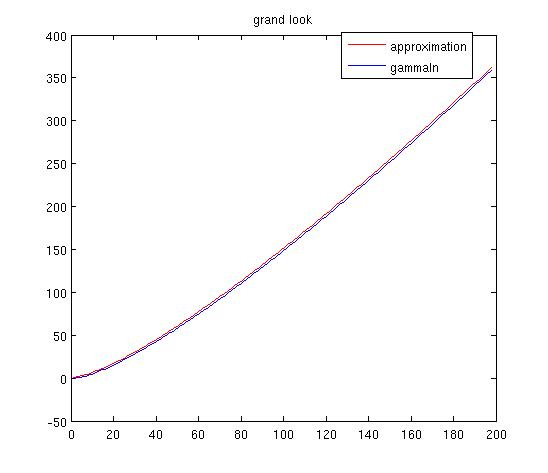
\includegraphics{g_ap1.jpg}} &
     \resizebox{40mm}{!}{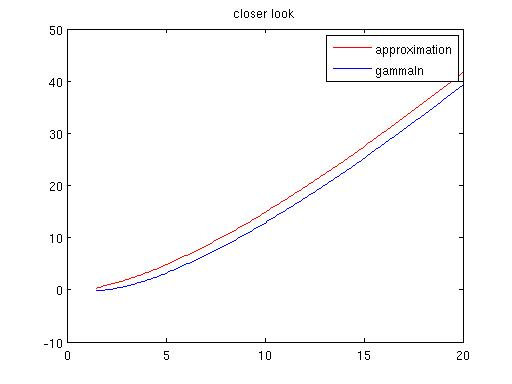
\includegraphics{g_ap2.jpg}}\\ 
        \end{tabular}
    \caption{left: Grand view; right: look closely}
    \label{fig:by:table} 
\end{figure}

\end{spacing}
\end{document}

%%%%%%%%%%%%%%%%%%%%%%%%%%%%%%%%%%%%%%%%%%%%%%%%%%%%%%%%%%%%%
